\section{Força de Casimir} 
Embora tenhamos obtido uma expressã analítica para a energia de vácuo, na equação \eqref{eq:casimirEnergyWithDelta}, nosso foco está em encontrar a força que age nas placas na direção z. A importância dessa quantidade decorre da possibilidade de analizar os termos de correções na equação \eqref{eq:casimirEnergyWithDelta} ao fazer uso de dados experimentais. Então calculemos a força de Casimir. Ela é dada por

\begin{equation}
\begin{aligned}
F_a(a,\tilde b)&=-\frac{\partial E(a,\tilde b)}{\partial a}=-\frac{L^2}{128\tilde b^4}\sum_{\delta=+,-}\left\{-\frac{3}{\pi^2}Li_5\!\left(e^{2i\pi\beta\delta}\right)\right.\\
&\left.+16\sum_{n=1}^{\infty}\sum_{q=1}^{\infty}\left[3\left(\frac{\tilde b(\delta n+\beta)}{aq}\right)^2K_2\!\left(\frac{a}{\tilde b}2\pi q|\delta n+\beta|\right)+2\pi\frac{\tilde b(\delta n+\beta)^3}{aq}K_1\!\left(\frac{a}{\tilde b}2\pi q|\delta n+\beta|\right)\right]\right\}\\
&-\frac{L^2}{8\tilde b^4}\sum_{q=1}^{\infty}\left[3\left(\frac{\tilde b\beta}{aq}\right)^2K_2\!\left(\frac{a}{\tilde b}2\pi q\beta\right)+2\pi\frac{\tilde b\beta^3}{aq}K_1\!\left(\frac{a}{\tilde b}2\pi q\beta\right)\right]. \label{eq:casimirForce}
\end{aligned}
\end{equation}

Esta força surge diretamente da energia de Casimir, equação \eqref{eq:casimirEnergyWithDelta}. Daí, podemos associar essa quantidade com a força de Casimir que age devido à inserção das condições de contorno do sistema. Note que no lado direito da equação \eqref{eq:casimirForce}, o primeiro termo refere-se à contribuição pura da dimensão extra compactificada, visto que não há influência de $a$. Perceba também que o último termo é devido à contribuição $n=0$ do somatório em $n$.

\begin{figure}[H]
\centering
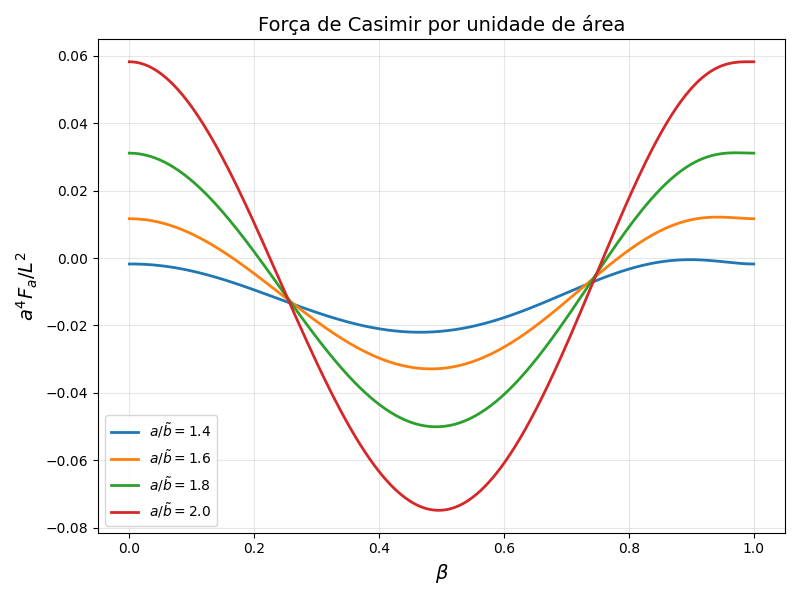
\includegraphics[width=0.8\textwidth]{Figure_3.png}
\caption{A densidade de energia $a^4F_a/L^2$ em função de $\beta$, para vários valores de $a/\tilde{b}$.}
\label{fig:force_beta}
\end{figure}

na figura \ref{fig:force_beta} plotamos a força de Casimir na equação \eqref{eq:casimirForce}, por unidade de área, em termos do parâmetro $\beta$. Podemos ver que $\beta$ tem uma influência clara na natureza da força (atrativa, repulsiva ou zero), assim como em sua intensidade. Comportamento parecido pode ser encontrado nas referências \cite{Farias2020, Farias2021}, reforçando que o parâmetro $\beta$ pode ser usado para controlar a natureza da força. 

\subsection{Valores específicos}

Consideremos agora os casos específicos das condições periódica ($\beta=0), 
